\section{Задача 1.25}
\subsection{Задание:}
Найти матрицу обратную к
$
	A =
	\begin{pmatrix}
		2 & 4 & 0 & 1 \\
		3 & -3 & 5 & 0 \\
		-1 & 0 & 1 & 1 \\
		2 & 1 & 1 & 0 \\
	\end{pmatrix}
$
\; методом алгебраических дополненй.
\subsection{Решение:}
Найдём $ \det A $ чтобы убедиться что $ \exists A^{-1} $:
\\[1em]
$
	\det A =
	\begin{vmatrix}
		2 & 4 & 0 & 1 \\
		3 & -3 & 5 & 0 \\
		-1 & 0 & 1 & 1 \\
		2 & 1 & 1 & 0 \\
	\end{vmatrix}
	=
	\begin{vmatrix}
		3 & 4 & -1 & 0 \\
		3 & -3 & 5 & 0 \\
		-1 & 0 & 1 & 1 \\
		2 & 1 & 1 & 0 \\
	\end{vmatrix}
	=
	\begin{vmatrix}
		3 & 4 & -1 & 0 \\
		3 & -3 & 5 & 0 \\
		-1 & 0 & 1 & 1 \\
		2 & 1 & 1 & 0 \\
	\end{vmatrix}
	=
	-
	\begin{vmatrix}
		3 & 4 & -1 \\
		3 & -3 & 5 \\
		2 & 1 & 1 \\
	\end{vmatrix}
	=
	5
$
\\[1em]
$ \det A \neq 0 \Rightarrow \exists A^{-1} = \dfrac{D^T}{\det A} $
\\[1em]
Вычислим матрицу алгебраических дополнений
$
	D =
	\begin{pmatrix}
		8 & -7 & -9 & 17 \\
		5 & -5 & -5 & 10 \\
		-8 & 7 & 9 & -12 \\
		-17 & 18 & 21 & -38 \\
	\end{pmatrix}
$
\\[1em]
$
	A^{-1} = \dfrac{D^T}{|A|} =
	\begin{pmatrix}
		8 & 5 & -8 & -17 \\
		-7 & -5 & 7 & 18 \\
		-9 & -5 & 9 & 21 \\
		17 & 10 & -12 & -38 \\
	\end{pmatrix}
	/ 5
	=
	\begin{pmatrix}
		\frac{8}{5} & 1 & -\frac{8}{5} & -\frac{17}{5} \\
		-\frac{7}{5} & -1 & \frac{7}{5} & \frac{18}{5} \\
		-\frac{9}{5} & -1 & \frac{9}{5} & \frac{21}{5} \\
		\frac{17}{5} & 2 & -\frac{12}{5} & -\frac{38}{5} \\
	\end{pmatrix}
$
\subsection{Компьютерная проверка в среде Wolfram Mathematica:}
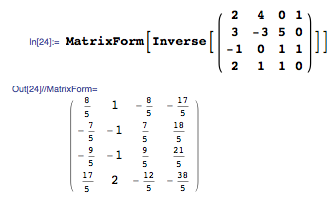
\includegraphics[scale=0.6]{task/1_25/screen1.png}
\subsection{Вывод:}
Компьютерная проверка показала что обратная матрица найдена верно.
